\documentclass[10pt,a4paper,twoside]{report}

% Add all packages and definitions.
\usepackage[utf8]{inputenc}
\usepackage[english]{babel}
\usepackage[margin=2.5cm]{geometry}
\usepackage[acronym]{glossaries}
\usepackage[pdftex]{hyperref}
\usepackage[style=ieee,url=false]{biblatex}
\usepackage{graphicx}
\usepackage{setspace}
\usepackage{csquotes}
\usepackage{xcolor}
\usepackage{subcaption}
\usepackage{epigraph}
\usepackage{minted}

\graphicspath{{images/}}


\renewcommand{\baselinestretch}{1.5}

% Table of Contents
\setcounter{tocdepth}{1}

% Use Arial font as default
%
\renewcommand{\rmdefault}{phv}
\renewcommand{\sfdefault}{phv}

\def\FontLn{% 16 pt normal
	\usefont{T1}{phv}{m}{n}\fontsize{16pt}{16pt}\selectfont}
\def\FontLb{% 16 pt bold
	\usefont{T1}{phv}{b}{n}\fontsize{16pt}{16pt}\selectfont}
\def\FontMn{% 14 pt normal
	\usefont{T1}{phv}{m}{n}\fontsize{14pt}{14pt}\selectfont}
\def\FontMb{% 14 pt bold
	\usefont{T1}{phv}{b}{n}\fontsize{14pt}{14pt}\selectfont}
\def\FontSn{% 12 pt normal
	\usefont{T1}{phv}{m}{n}\fontsize{12pt}{12pt}\selectfont}

% References

\addbibresource{references/misc.bib}
\addbibresource{references/access_control.bib}
\addbibresource{references/blockchain.bib}
\addbibresource{references/evaluation.bib}
\addbibresource{references/methods.bib}

\AtEveryBibitem{%
	\clearfield{note}%
}


\begin{document}

\pagestyle{empty}

% Cover
% IST Logo - Signature A

\includegraphics[bb=9.5cm 11cm 0cm 0cm,scale=0.29]{IST_A_RGB_POS.png}

\hspace*{9.5cm}
\includegraphics[bb=0cm 0cm 0cm 1.5cm, scale=0.6]{IG_AssinaturaEletronica_sobre_fundo_branco-300x82.jpg}

\begin{center}
    \vspace{5cm}
    {\FontLb Exploring Permissioned Blockchains for Decentralizing Access Control} \\
    \vspace{0.3cm}
    {\FontMn Application to an Educational Certificates Use Case} \\
    \vspace{1.5cm}  
    {\FontMb Hugo Figueiredo Caramelo Santos Martins} \\
    \vspace{1.5cm}
    {\FontSn Thesis to obtain the Master of Science Degree in} \\
    \vspace{0.3cm}
    {\FontLb Information and Enterprise Systems} \\
    \vspace{1.5cm}
    {\FontSn %
        \begin{tabular}{ll}
            Supervisor: Sérgio Luís Proença Duarte Guerreiro
        \end{tabular} } \\
    \vspace{1.5cm}
    {\FontMb Examination Committee} \\
    \vspace{0.3cm}
    {\FontSn %
        \begin{tabular}{c}
            Chairperson: Miguel Leitão Bignolas Mira da Silva  \\ 
            Supervisor: Sérgio Luís Proença Duarte Guerreiro \\ 
            Member of the Committee: Miguel Nuno Dias Alves Pupo Correia
        \end{tabular} } \\
    \vspace*{\fill}
    {\FontMb October 2018}
\end{center}
\cleardoublepage

\pagestyle{plain}
\pagenumbering{roman}

% Acknowledgements
\chapter*{Acknowledgments}

I am grateful to Prof. Sérgio Guerreiro, my supervisor, for his guidance, patient and support, through the course of this thesis. I am grateful to Filipe Apolinário, João Pereira and Andreia Silva for fruitful discussions that kept me motivated and focused on doing more and better. I am grateful to my parents, for the help and discussions provided during this thesis, for the opportunities and upbringing they gave me that enabled this achievement. I am grateful to Mariana Sequeira for her support, patience and essentially not allowing me to give up. This thesis would not have been completed without her.
\addcontentsline{toc}{chapter}{Acknowledgments}
\cleardoublepage{\tiny}

% Resumo
\vspace*{\fill}

\begin{center}
	\section*{Resumo}
	\textcolor{red}{TODO}
\end{center}

\vspace*{\fill}
\addcontentsline{toc}{chapter}{Resumo}
\cleardoublepage

% Abstract
\section*{Abstract}

Protecting sensitive or private information is of the utmost importance. Information breaches, and sharing of sensitive information can have serious legal, reputation and financial impacts for individuals and organizations. At the same time, our technological landscape is getting more and more complex and distributed, being increasingly hard to protect information. A particular demonstration of this situation can be found in institutions providing certificates of accomplishment, such as Universities, who have been increasing efforts to shut down fake certificate generators online, while working in an environment where validation of credentials is essential, yet, done sporadically and requiring interactions between several parties. This situation exposes a gap between the needs of modern, complex distributed environments, in regards to control of access to information, and the level to which classic access control solutions can fulfill those needs. This thesis explores permissioned blockchains as technological vehicles for decentralizing access control, applied to this specific use case. This thesis proposes \texttt{Blocked}, a system that allows decentralized access control, through a permissioned blockchain, for issuing, sharing and managing educational certificates. An evaluation of this system demonstrates that it can be considered a suitable access control system, with improvements over the existing decentralized solutions for the same problem.

\vfill

\noindent \textbf{Keywords:} Access Control, Security, Privacy, Blockchain, Decentralized Systems

\addcontentsline{toc}{chapter}{Abstract}
\cleardoublepage

% TOC
\tableofcontents
\cleardoublepage

% List of tables
\phantomsection
\addcontentsline{toc}{chapter}{\listtablename}
\listoftables
\cleardoublepage

% List of figures
\phantomsection
\addcontentsline{toc}{chapter}{\listfigurename}
% Generate list
\listoffigures
\cleardoublepage

% Add entry in the table of contents as section
\phantomsection
\addcontentsline{toc}{chapter}{Glossary}
\printglossary[type=\acronymtype,title=\glossaryname]
\cleardoublepage

\setcounter{page}{1}
\pagenumbering{arabic}

% -------------------------------------------------------
% Chapters
% -------------------------------------------------------

\chapter{Introduction}
\label{chap:intro}

\epigraph{\textit{The essence of the independent mind lies not in what it thinks, but in how it thinks.}}{Christopher Hitchens \cite{hitchens_letters_2009}}

\section{Motivation}

Our society is built on top of and quite dependent on centralized webs of trust. We share our personal information on a daily basis, either voluntarily by sharing it with trusted entities, such as banks and governments, or involuntarily, by making use of applications, or visiting websites, that collect our personal information. The institutions that form those webs of trust have sadly failed short of their responsibilities, on numerous occasions. Three interesting challenges emerge from this situation: \emph{(i)} are individuals, on their own, or as a collective, capable of enhancing their own privacy, through the use of technology \emph{(ii)} are there enhanced ways of sharing personal information, in a private and secure fashion, and \emph{(iii)} could breaking this centralization (\textit{e.g.}, decentralization) be a solution for improving the current \textit{status quo}?

At the same time, the amount of information humans have to process on a daily basis is enormous. It is also increasing very rapidly. This situation has created an environment in which it is becoming increasingly difficult for people to validate whether a piece of information is truthful or if it is incorrect. An example of this, exposed through media outlets, is the \text{misinformation war} ocurring, at the moment, throughout social media. It is also a topic of interest for researchers who have gone through lengths to study the problem of spread of news online \cite{vosoughi_spread_2018}. To provide another example, institutions that provide certifications of accomplishment, such as Universities, are also starting to become affected by this spread of falsehood, regarding digital efforts. There’s an increasing effort to shutdown fake certificate websites \cite{camilla_telegraph} such as RealisticDiplomas \cite{RealisticDiplomas} or DiplomaCompany \cite{DiplomaCompany}, among others, and, recently, there have surged news of falsified PhD diplomas being used.This example comes from a completely different perspective than the previous examples - \textit{fake news} - but shares some of same consequences: \emph{(i)} it affects the credibility of trusted institutions, \emph{(ii)} it impacts the outcome of certain situations due to a falsehood and \emph{(iii)} it can have serious legal and financial impacts for society.

To add complexity to this ecosystem, the information created is being offloaded, ever more rapidly, to third-party systems and entities, in the form of cloud storage, which requires users to manage access to it. Users are also getting more perceptive about the importance of being able to control what stored data entities have access to or not. \textcolor{red}{end-to-end encryption}, \textcolor{red}{data breaches} 

We have presented three independent topics that are becoming increasingly relevant: \textit{privacy}, \textit{verification} and \textit{access control}. These are societal issues which are gaining relevance in the public sphere but they are also, at the same time, organizational issues in way by which corporations can adapt and improve on these problems.

\section{Objectives}

As presented above, there's an increasing gap between the necessities of modern, and complex, distributed environments, in regards to control of access to data and resources, and the level to which classical access control solutions can fulfill those needs.

This research, presented in the context of what has been described above, aims to deepen the existing knowledge, with regards to access control models, and implementations, in complex and distributed technological environments, through an analysis of existing literature, a new approach and an implementation. We aim to provide a starting point, for research that is more focused on enterprise-level application of private decentralized access control solutions, over theoretical approaches. \textbf{Specifically, we want, with this thesis, to propose an inherently decentralized approach, focused on distributed file systems, that can showcase improved traceability, reliability, and security over existing approaches.} This approach aligns, from a business perspective with the practice of enterprise content management, at the document management level, within organizations. Our approach is based on using blockchain-based technologies (\cite{nakamoto_bitcoin:_2008}, \cite{buterin_next-generation_2013},\cite{wood_ethereum:_2014}) as the backbone of decentralized access control, leveraging blockchain's very own characteristics. A key aspect of our proposal, apart from being fully decentralized, is the focus on the use of private blockchains instead of using public ones (e.g. Bitcoin's - \cite{nakamoto_bitcoin:_2008} - or Ethereum's - \cite{buterin_next-generation_2013}, \cite{wood_ethereum:_2014}), mainly due to the fact that private blockchains are more suitable for enterprise environments.

Finally, we intend to produce further knowledge, in the research field, in the form of book chapters, paper submissions and poster submissions, to share the body of knowledge acquired over the course of the thesis and validate this research's results with the scientific community.

\section{Contributions}
\label{sec:contributions}

After describing the objectives of the presented research, it is now relevant to summarize, concretely, what are the contributions made in this thesis. As such, this thesis makes the following contributions:

\begin{itemize}
	\item a chapter in an edited book, describing access control challenges in enterprise ecosystems and possible solutions through blockchain-based technologies \cite{bryan_christiansen_access_2018}, whose main content was derived from the extensive analysis of the state-of-art presented in this thesis, description and motivation of the problem;
	\item an access control model based on ACLs and cryptography, to be used on enhancing access control on data stored inside a blockchain, as well as, a baseline framework for storing data and access control policies inside a blockchain, specifically on a permissioned blockchain built with Hyperledger Sawtooth;
	\item a proof-of-concept implementation for storing and managing Educational Certificates, and access control policies, based on the proposed models and framework, including a Transaction Processor that can be used, or extended, for Hyperledger Sawtooth, on different configurations and implementations, to process transactions, relevant to this domain;
	\item an exploratory statistical study, based on an online questionnaire, of user's perception of blockchain in terms of security and complexity, applied to an Educational Certificates use case;
	\item an evaluation on the viability of permissioned blockchains for decentralizing access control and enhancing data ownership, in the context of Educational Certificates issuance, sharing and verification.
\end{itemize}

Apart from these concrete contributions, components of the research presented in this thesis have been submitted as conference research papers for \emph{(i)} \textit{\gls{acmsac19}} and \emph{(ii)} \textcolor{red}{SECOND CONFERENCE PAPER}. The submission for \gls{acmsac19} focused on the work conducted throughout Chapter \ref{chap:study}, while the submission for \textcolor{red}{SECOND CONFERENCE PAPER} focused on the work conducted throughout Chapter \ref{chap:implementation} and Chapter \ref{chap:evaluation}. As a related achievement, due to the work conducted during this thesis, the author has been invited to peer-review research for \textit{\glsdesc{hicss52}}, on the topic of the \textit{Transformationl Impact of Blockchain}.

\section{Document Outline}

This document is structured throughout 7 chapters. After this chapter, we have Chapter \ref{chap:related} outlines some of the necessary background to this thesis, surveys the existing state-of-art and further motivates this thesis by pointing a research gap in the existing research. Chapter \ref{chap:methods} describes and motivates the methodology used throughout the research, while exposing the intersection between the chosen methodology and the chapters in this thesis. Chapter \ref{chap:study} presents a study, based on data collected through an online questionnaire with the aim of exploring the perception of users about the security and complexity of blockchains, which is a component of the solution presented in this thesis. Chapter \ref{chap:implementation} describes the implementation of the prototype developed, including the access control framework, selected technologies, design and architectural decisions. Chapter \ref{chap:evaluation} presents the evaluations of our prototype and discusses the utility of our artifcats through a series of analytical, experimental and descriptive methods. The evaluation methodology has been described previously in Chapter \ref{chap:methods}. Finally, Chapter \ref{chap:conclusion} analyzes what has been achieved in this thesis and where future research can be directed towards by discussing limitations and unexplored paths of research.

\cleardoublepage

\chapter{Related Work}
\label{chap:related}

In this chapter we present some relevant background and work that is related with this thesis. Due to the broad nature of our research problem, as described in the previous chapter, there's a need to review several different areas of interest. We start by reviewing, in Section \ref{sec:related-ac}, existing literature on \gls{ac} models and applications, discussing how they related to this research and highlighting the chosen models for our use case. Section \ref{sec:related-blockchain} reviews different blockchain approaches, dissecting their components, and describes existing literature on blockchain applications. Finally, Section \ref{sec:related-ec} reviews some of the work done on the topic of Educational Certificates, which is the use case of focus in this thesis. By the end of this chapter, it should be possible to realize how these concepts, and existing literature, relate to the core contributions of thesis. It should also be possible to contextualize our core research within the existing literature and, at the same time, lay out the necessary concepts to understand the forthcoming chapters.

\section{Access Control}
\label{sec:related-ac}

\glsdesc{ac} has been a core component in every technology evolution and continues to be as relevant today. It has always played a central role in technology because information is a valuable asset that must be protected from prying hands. Due to that fact, both governments and corporations have spent resources on developing \gls{ac} models and instantiations, while academia produced a broad spectrum of literature on the topic. Said literature has been produced with all sorts of approaches, from the purely theoretical to implementation-based approaches. Nonetheless, no matter what has been produced and developed previously, there are always new challenges to be faced and, with every new evolution, a new challenge emerges, which has led the field to be one of extensive study ever since the beginnings of the computer age. As more sensitive data is shared and stored by third-parties, the relevance of \gls{ac} is only increasing, rather than decreasing, creating an optimal context for researchers to be able to developed interesting new research that solves important problems.

\subsection{\glsdesc{mac}}

\glsdesc{mac} is a keystone \gls{ac} approach characterized by embedding access control policies inside systems rather than in external sources, transforming the policy into an unchangeable entity \cite[23]{biba_integrity_1977}. To help clarify, let us imagine an application, written in a given programming language, which has access to a given set of resources. Using \gls{mac}, the access control policies for a subject to access each of the resources would have to be embedded - hard-coded through programming - into the application itself such that any adjustment to the access control policies would require an adjustment to the application itself. This approach emerged in the early stages of \gls{ac} research, in the 1970s, when research on this topic was very focused for military applications \cite{sandhu_lattice-based_1993}.

\citeauthor{sandhu_lattice-based_1993} provides an overview of the existing foundational models following this approach \cite{sandhu_lattice-based_1993}: the Bell-LaPadula model \cite{bell_secure_1973} and the Biba model \cite{biba_integrity_1977}, as well as \citeauthor{denning_lattice_1976}'s axioms for information flow policies \cite{denning_lattice_1976}.

\subsection{\glsdesc{dac}}

A more flexible approach, albeit potentially less secure, is \glsdesc{dac}. \citeauthor{sandhu_lattice-based_1993} refers to \gls{dac} as \emph{"inadequate to enforce information flow"} \cite[8]{sandhu_lattice-based_1993}, due to its lack of constraints on copying information. \gls{dac} is characterized by allowing policies to be defined dinamically, contrary to the inherently static policies provided with \gls{mac} \cite[23]{biba_integrity_1977}. With \gls{dac}, policy enforcement is achieved by comparing a subject and its associated groups with the resources’ group permissions. In other words, validation is performed to answer the following question: is the subject, or a group the subject belongs to, allowed access to a specific resource?

\gls{dac} models are intrinsically related with the concept of an \emph{access matrix} \cite{graham_protection:_1972, lampson_protection_1974}. Access matrices are defined by a matrix composed of both objects and subjects – subjects which can
be replaced by access domains or groups – that define a system’s access control policy. During policy
enforcement, access to an object is allowed if the intersection between subject and object bears a policy
that allows access to said object. Along with the models proposed by \citeauthor{graham_protection:_1972} and \citeauthor{lampson_protection_1974}, there's another foundational model that implements this concept known as the \gls{hru} model \cite{harrison_protection_1976}. More recent models have been proposed to overcome a set of undecidable cases when performing policy enforcement, with \gls{hru}, which left it vulnerable as an access control model \cite{sandhu_schematic_1988, sandhu_typed_1992}.

\subsection{\glsdesc{rbac}}

\glsdesc{rbac} emerges a commercially focused approach to access control, contrary to \gls{dac} and \gls{mac} which were predomenantely government and military focused \cite{ferraiolo_role-based_1992}. RBAC introduced the concept of roles as an intermediary abstraction between the object and subjects, in access control. With RBAC, policy definition was composed of three elements: subjects, objects, and roles \cite{ferraiolo_role-based_1992}. In this sense, RBAC is already different from the solutions as described above. With RBAC, roles are defined as a function of, for example, employee’s job titles. Each subject is assigned a role and each object is allowed access to a set of roles. During policy enforcement, the validation performed is if the subject is a member of the defined roles to which the object allows access. RBAC made policy management easier and it was better suited for application systems that were commercially-focused instead of the military-based applications for which access control had been developed \cite{ferraiolo_role-based_1995}. The reason for this suitability is due to the manner in which organizations are usually structured. Organizations, unlike the military, have employees assigned specific business roles and functions. Those roles carry with them a set of tasks and permissions that every employee, assigned to that role, must possess. Organizations can easily have dozens, hundreds or thousands of employees which makes managing policy at an individual level, painstakingly difficult. By abstracting individual employees into sets of roles, the set of definitions that are needed decreases dramatically.

Apart from the foundational model, proposed by \citeauthor{ferraiolo_role-based_1992}, in \citeyear{ferraiolo_role-based_1992}, other models soon emerged such that a family of \gls{rbac} reference models was specified, known as RBAC96 \cite{sandhu_role-based_1996}. Aside from providing a formal definition of 4 models, with the base model being the one defined previously \cite{ferraiolo_role-based_1992}, this work also added the ability for roles to have hierarchy and constraints attached to them, independently or at the same time. A wide array of variantions to \gls{rbac} exist with temporal constraints \cite{bertino_supporting_1996, bertino_temporal_1996} and periodic constraints \cite{bertino_access_1998}. Other variations have evoled into indenpendent concepts that rely on the \gls{rbac} foundations such as \gls{trbac} \cite{bertino_trbac:_2000}, \gls{erbac} \cite{bonatti_erbac:_2013}, \gls{grbac} \cite{covington_generalized_2000}, \gls{tmac} \cite{thomas_team-based_1997}, \gls{lrbac} \cite{ray_lrbac:_2006} and \gls{geo-rbac} \cite{damiani_georbac:_2007}. A lot more variants of the \gls{rbac} model exist with these being but a few examples. Apart from variations on the model, research has been performed on proving that \gls{rbac} constructs are sufficiently expressive to replace both \gls{dac} and \gls{mac}. This research because it shows how to perform upgrades on legacy systems, using \gls{dac} or \gls{mac}, to mode modern, or potentially suitable, access control models.

\subsection{\glsdesc{abac}}

There's one thing the proliferation of \gls{rbac} variations uncovers which is that the world is getting increasingly more broad in the necessities of access control, with small variations to access control being dependent either on the context of the problem domain, or the context of the system in which it is being implemented. In \gls{abac}, different from what has been described above in the other approaches, access control is provided by containing a specific element, apart from subjects, objects and roles – attributes. \gls{abac} utilizes subject and object attributes (or environment attributes) in policy definition as well as in policy enforcement \cite{hu_guide_2014}. The usage of attributes, in access control policy definition and enforcement, increases the expressiveness of policies and allows policy enforcement to be based more on dynamic data - increasing the effectiveness of access control.

Given the flexible and case-to-case nature of \gls{abac}, formally defining a generalized model is not easy, like the ones presented for \gls{dac}, \gls{mac} and \gls{rbac}. \citeauthor{hu_guide_2014} have attempted a formal definition from previous definitions \cite{wang_logic-based_2004, yuan_attributed_2005, cruz_constraint_2009}. Models for a variety of use cases have been proposed such as: an attribute-based access matrix \cite{zhang_attribute-based_2005}, \gls{abac} for webservices \cite{yuan_attributed_2005}, attribute-based encryption \cite{goyal_attribute-based_2006, wang_hierarchical_2010}, grid computing \cite{lang_flexible_2009}, \gls{abac} applications on \gls{rbac} \cite{kuhn_adding_2010}, cloud computing \cite{wan_hasbe:_2012, yang_attribute-based_2013}, \gls{iot} \cite{bhatt_access_2017, ouaddah_access_2017} and data sharing \cite{yu_attribute_2010}. There's been an attempt at unifying \gls{abac} into a model that could replace the previous models \cite{jin_unified_2012}, much like we have described for \gls{rbac}.

\subsection{Cryptography Access Control}

A research topic which aligns so deeply with our current digital environment, such as the application of cryptographic methods in Access Control, finds early research in \cite{akl_cryptographic_1983}, published in 1983, with the proposal of a cryptographic solution for access control in organizations that are structured hierarchically. This research presents a system, which takes advantage of cryptographic keys, to allow a principal the derivation of cryptographic keys from each of the cryptographic keys below it, in a hierarchy. This capability allows an implemented system, in a structurally hierarchical organization, to be able to interpret security policies based solely on cryptographic methods.

Later, MacKinnon et al. suggest an optimal algorithm for the distribution of cryptographic keys, in \cite{mackinnon_optimal_1985}, precisely, in the context of hierarchical access control. This way of managing access control was also studied in \cite{sandhu_cryptographic_1988}. In it, Sandhu proposes a solution that is different from what had been presented in \cite{akl_cryptographic_1983}. MacKinnon et al., Akl and Taylor and Sandhu's research was an evolution over Denning's initial research, in 1981, in the area of master cryptographic keys \cite{denning_master_1981}, this concept allowed the derivation of key cryptographic keys . In this context, the studies carried out in the 1970s and early 1980s laid the foundations for the more complex, generic models set forth later.

This historical basis is not only interesting as a subject of study, but also important for contextualizing the problem. The reason for this is that research initialized in the 1970s continues to this day, becoming increasingly relevant. From the studies carried out during the 1970s and the early 1980s, new research subjects, and developments from the earlier ones, began to emerge. Chick and Tavares presented a solution, with greater flexibility, to use master cryptographic keys \cite{brassard_flexible_1990} in access control, evolving the initial works in \cite{akl_cryptographic_1983} and \cite{denning_master_1981}. Park and Sandhu continue to develop their research applying digital certificates in access control, in \cite{park_binding_2000}, in 2000. In \cite{miklau_controlling_2003}, Miklau and Suciu, demonstrate an interesting implementation that uses cryptography to control access to XML documents.

More recent research has also evolved the cryptographic use in access control, building on the blocks that have been proposed earlier \cite{di_vimercati_over-encryption:_2007}. Other works overlap with \gls{abac} \cite{wan_hasbe:_2012, ruj_privacy_2012, wang_hierarchical_2010, goyal_attribute-based_2006, harrington_cryptographic_2003}.

\subsection{Decentralized Access Control}

The study of access control in distributed systems has spanned several decades since the early developments of distributed systems through grid and cloud computing and cloud systems. Some of the beginning studies developed in the field of access control in decentralized environments \cite{karger_non-discretionary_1977} encompass much of the knowledge to date. As with initial research regarding access control models, \citeauthor{karger_non-discretionary_1977} presents the challenges in distributed systems when applying MAC to a decentralized system. It recognizes that not all algorithms that guarantee access control in centralized systems can be easily mapped to a decentralized system, thus presenting a new way to work with lattice-based access control models that can be used in decentralized systems.

\citeauthor{moffett_specifying_1990} proposed a specification for the implementation of discretionary
access control in distributed systems. In this research, the concept of domains, groups of objects and
access rules were introduced as a way of helping structure the way access control is managed in a highly
distributed and complex system. This work evolved, in part, from \citeauthor{satyanarayanan_integrating_1989} on security in complex distributed systems. Research over the Andrew system \cite{satyanarayanan_integrating_1989} explored how to introduce access control in complex distributed systems.\citeauthor{sandhu_implementation_1992}, presented enhancements over Sandhu’s initial Typed Access Matrix model \cite{sandhu_typed_1992}. This research proposed a simpler TAM, called SO-TAM, that made it easier to implement Typed Access Matrix, in distributed environments, as well as demonstrated the usage of digital certificates in access Control.

\citeauthor{johnston_authorization_1998} present a mechanism for access control in distributed
systems. The system described leverages the research and capacity of digital certificates to allow access
control in distributed systems. This research represents the evolution in the area of access control in
distributed systems and revalidates its relevance. \citeauthor{sandhu_decentralized_1998} present the decentralization of access control management in RBAC models, in web-based systems. This research presents a way to try and decentralize the management of access control, but it still does not decentralize the policy engine behind the access control. \citeauthor{sandhu_decentralized_1998} was an enhancement over a previous specification \cite{barkley_role_1997}. The research presented \cite{sandhu_decentralized_1998} was evolved through the use of X.509 certificates \cite{park_smart_1999} and \citeauthor{park_role-based_2001} return to examine this research.

\citeauthor{harrington_cryptographic_2003} note that one of the main problems in the area of access control is the centralization of the reference monitors, and present a proposal for a cryptographic access control system, which is inherently distributed but not completely decentralized. This research evolves what has been presented earlier \cite{satyanarayanan_integrating_1989}. \citeauthor{park_role-based_2003} demonstrate the application of the RBAC model in peer-to-peer environments, which is an evolution towards a more complete decentralization of access control. \citeauthor{abiteboul_electronic_2004} present the implementation of a distributed system of access to confidential patient data, in a distributed way, through XML data that presents an evolution over the research produced earlier \cite{damiani_fine-grained_2002}.

\citeauthor{bhatti_x-gtrbac_2004} present a system - X-GTRBAC - for access control management, in GTRBAC model \cite{joshi_generalized_2005}, over decentralized environments. \citeauthor{chakraborty_trustbac:_2006} present a new access control model, called TrustBAC, to address a problem identified in RBAC: difficulty in assigning roles to subjects in decentralized systems, due to the fact that, in this type of systems, identities are often not known a priori and the “user population is dynamic”.

With the proliferation of decentralized systems, developments in the area of access control continue
to emerge. \citeauthor{ruj_dacc:_2011} present a new algorithm and model for the access control in clouds by expanding on the cryptographic research previously published. \citeauthor{calero_toward_2010} propose a system for the same effect based on the RBAC model. This model intends to describe a suitable architecture for an access control system for cloud computing. \citeauthor{yu_achieving_2010} present their model for access control in cloud computing, which is related to previous research \cite{calero_toward_2010}. Recently, a number of attribute-based access control models have been developed. \citeauthor{ruj_decentralized_2014} present research on access control in decentralized systems in which the identity of the principal is unknown. The research presented \cite{ruj_decentralized_2014} extends what had already been done by \citeauthor{ruj_privacy_2012}.

\subsection{Discussion}

\textcolor{red}{TODO}

\section{Blockchain}
\label{sec:related-blockchain}

\subsection{Primer on Blockchains}

 technologies emerged as a supporting technology for the cryptocurrency Bitcoin, although under a different name \cite{nakamoto_bitcoin:_2008}. \citeauthor{nakamoto_bitcoin:_2008}'s contribution was to solve the \textit{double spending problem} without using a trusted central authority. For this, time stamping servers were used, which use the concept of blocks of hashes, with each hash having a reference to the previous block, and a modification of an existing proof-of-work algorithm \cite{back_hashcash_2002}, initially developed to mitigate Denial of Service attacks. Thus, the name for what we now call blockchains comes from the fact that, simply put, they can be represented as chains of blocks, with references to previous blocks. The concept proposed by \citeauthor{nakamoto_bitcoin:_2008} was then to have transactions of the cryptocurrency Bitcoin broadcast to all nodes on the network, after which each node would process that transaction and try to find a proof-of-work. When a node was successful, it would broadcast its block to all other nodes, and that block would be accepted only if all previous transactions in it were valid and not spent before.

In essence, a blockchain can be perceived as a decentralized transaction ledger, with no central authority and no single point of failure. This ledger is maintained by a chain of blocks, that represent the transactions, and the creation of new blocks is managed through consensus' protocols. Until now, the concept of a blockchain doesn't have a formal definition but several definitions have been presented through new research. In \cite{buterin_next-generation_2013}, \citeauthor{buterin_next-generation_2013} suggests, appropriately, that one of the most revolutionizing aspects of the Bitcoin experiment is not the decentralized cryptocurrency, and the financial implications it might have, but rather the fact that this new blockchain concept can be \textit{"a tool of distributed consensus"} and presents \textit{Ethereum} as a platform for building decentralized applications, and not only cryptocurrencies. As predicted by \citeauthor{buterin_next-generation_2013}, and later described by \citeauthor{pilkington_blockchain_2016}, in \cite{pilkington_blockchain_2016}, blockchain technology, while still being at the very core of cryptocurrencies, started moving away and dwelling further into other applications. In \cite{pilkington_blockchain_2016} we can blockchains adoption started moving from, not only, Ethereum, or Ripple, towards more practical applications such as identity providers, voting systems, supply chain alternatives for enhanced transparency or banking applications. At the same time other research has pointed towards different possible applications of blockchain technology, other than cryptocurrencies (\cite{crosby_blockchain_2016}, \cite{underwood_blockchain_2016}, \cite{yermack_corporate_2017}, \cite{xu_blockchain_2016}).

\subsection{Applications}

While the technology itself keeps evolving and under analysis (\cite{eyal_bitcoin-ng:_2016}, \cite{wang_research_2018}, \cite{gervais_security_2016}, \cite{lin_survey_2017}), and the entire concept of Bitcoin is already heavily based on previous academic literature \cite{narayanan_bitcoins_2017}, we are only now starting to apply this technology to practical problems of our society. One of those issues, and one that has currently been the focus of major media attention, as well as in the academic environment, is the area of Information Security. Given its decentralizing nature, as well as its cryptographic background, blockchains have started to gather attention for their potential applications at the level of access control, privacy and security in general. This happens due to the increasingly distributed and federated environments in which we now live, such as the Internet of Things, which call for different approaches and concepts, when considering how to more effectively to secure them.

Research over using blockchain to resolve problems with \textit{data ownership} and privacy has been conducted in \cite{zyskind_decentralizing_2015}, \cite{liang_provchain:_2017} and \cite{yue_healthcare_2016}. It has also been researched as a way to enhance security and decentralization in content distribution \cite{fotiou_decentralized_2016}. At the same time, blockchain has also been researched as, potentially, an application for enhanced security of IoT infrastructure, in \cite{dorri_blockchain_2016}, \cite{dorri_blockchain_2017} and \cite{ouaddah_access_2017}. Furthermore, on the factor of access control and identity management, there's been some research developed by \citeauthor{augot_identity_2017} in \cite{augot_identity_2017}, as well as \citeauthor{maesa_blockchain_2017} in \cite{maesa_blockchain_2017}. In \cite{ouaddah_fairaccess:_2017}, an overlap between access control and IoT was researched, in which blockchain enhanced access control on IoT infrastructure. Finally, there's been research on applying blockchain technology into securing smart cities \cite{biswas_securing_2016}, decentralized private voting systems \cite{sheer_hardwick_e-voting_2018} and securing credit reporting \cite{kafshdar_goharshady_secure_2018}.

\subsection{Discussion}

\textcolor{red}{TODO}

\section{Educational Certificates}
\label{sec:related-ec}

MIT's Media Lab Learning Initiative, along with Learning Machine, have conducted research, \textit{Digital Certificates Project} \cite{MITCertificates}, in 2015, on this subject. This research developed the first prototype, to the authors' knowledge, that allowed to create an ecosystem for issuing and sharing educational certificates, based on blockchains. Some certificates generated based on this prototype are still accessible \cite{MITCertificatesBootcamp}. \textit{Digital Certificates Project}, initially focused on issuing digital certifications for educational purposes, later spun \textit{BlockCerts} \cite{Blockcerts}, which expanded the issuing of certificates from educational certificates to more generic use cases. \textit{BlockCerts} claims to be \textit{"The Open Standard For Blockchain Credentials"} and, contrary to what had been developed for \textit{Digital Certificates Project}, it includes a more robust ecosystem, based on the open-sourced code of the initial prototype. \textit{BlockCerts} now includes libraries, apps and tools to allow the development of decentralized  applications for issuing and sharing digital (educational) certificates.

Although \textit{BlockCerts} is an effort to standardize the development of decentralized applications for these purposes, it currently lacks some functionality - some of it defined in its Roadmap - such as: \emph{(i)} only works with Bitcoin and Ethereum. This means there's a lack of support for additional public blockchains or federated blockchains; \emph{(ii)} revocation is highly dependent on the issuer and there's a lack of access control capabilities for the recipient of the certificate; \emph{(iii)} uses the same approach as cryptocurrencies - the wallet concept - to manage the issuing and sharing of the certificates.

As with any new technology, there's a lot of innovation space. \textit{BlockCerts} has growing a strong open-source community and an ecosystem that enables some existing gaps to be closed. It also helps to state the relevance of the issue at hand, presented in this section.

\section{Summary}

\textcolor{red}{TODO}


\cleardoublepage

\chapter{Methodology}
\label{chap:methods}

In previous sections (Chapter \ref{chap:intro} and Chapter \ref{chap:related}) we motivate our thesis, by analyzing the existing literature, defining and motivating a specific research problem, setting out the objectives and describing the contributions made by this research. It is now relevant to explain the methodology used in our research and the factors that contributed to choosing it. We will also describe how the various sections of this thesis intersect and fit into the chosen methodology, through the adoption of the same presentation model described by the methodology's authors.

\gls{is} has devoted considerable effort to studying methods and frameworks for IS research. Currently, two main paradigms characterize IS research: \gls{bs} and \gls{ds} \cite[76]{hevner_design_2004}. After carefully evaluating existing reference literature, such as \cite{hevner_design_2004}, \cite{march_design_1995}, \cite{winter_design_2008} or \cite{peffers_design_2007}, a suitable research methodology would be to conduct our research based on the guidelines for \gls{dsr}, as it is a common and accepted practice in \gls{is} research.

In their seminal paper, \citeauthor{march_design_1995} \cite{march_design_1995} define a \gls{ds} research framework by applying natural science methodologies to the study of \gls{is}, with the purpose of maximizing research utility, contrasting with the natural sciences' view of research for truth (\cite[80]{hevner_design_2004}, \cite[253]{march_design_1995}). They achieve that by creating a framework consisting of a two-dimensional matrix: research outputs and research activities \cite[255]{march_design_1995}. Research outputs are composed by \textit{constructs}, \textit{models}, \textit{methods} and \textit{instantiations}. Research activities, on the other hand, are composed by processes such as \textit{build} and \textit{evaluate}. Research outputs, also known as \textit{artifacts}, are created with the purpose of solving a specific problem that has yet to be solved \cite[78]{hevner_design_2004}, while research activities are the processes by which those are artifacts are designed to meet a criteria \cite[79--80]{hevner_design_2004}. \citeauthor{hevner_design_2004} \cite{hevner_design_2004} argued that, in fact, truth and utility are inseparable \cite[80]{hevner_design_2004}. This statement is the basis for their approach, which extends the original \gls{dsr} framework \cite{march_design_1995} presented by \citeauthor{march_design_1995} \cite{march_design_1995}, by setting the following practical guidelines: \emph{(i)} Design as an Artifact, \emph{(ii)} Problem Relevance, \emph{(iii)} Design Evaluation, \emph{(iv)} Research Contribution, \emph{(v)} Research Rigor, \emph{(vi)} Design as a Search Process and \emph{(vii)} Communication of Research. Summarizing, \gls{dsr} requires the creation of a novel, innovative, purposeful artifact, that is formally defined, for application on a specific problem domain, created through a search process to find an effective solution and, finally, communicated effectively to the community \cite[82]{hevner_design_2004}.

\citeauthor{peffers_design_2007} \cite{peffers_design_2007} present a \gls{dsrm}, extending previous research \cite{march_design_1995, hevner_design_2004}, \textit{"for the production and presentation of \gls{ds} research in \gls{is}"} \cite[3]{peffers_design_2007}. This research expanded on previous concepts by proposing a missing procedure \cite[7]{peffers_design_2007} that would connect both the principles and practical guidelines existing in \gls{ds} to create a formal research methodology. With that in mind, they have proposed a series of activities that form a process by which to conduct \gls{dsr}: \emph{(i)} Problem Identification and Motivation, \emph{(ii)} Define the Objectives for a Solution, \emph{(iii)} Design and Development, \emph{(iv)} Demonstration, \emph{(v)} Evaluation and \emph{(vi)} Communication. This set of activities aligns well with the practical rules proposed by \citeauthor{hevner_design_2004} \cite{hevner_design_2004} and, as \citeauthor{peffers_design_2007} argue, with most of the literature conducted thus far. Although the procedure is presented sequentially, the authors point out that \textit{"there is no expectation that researchers would always proceed in sequential order from activity one through activity six"} \cite[14]{peffers_design_2007}, which provides flexibility while conducting research while, at the same time, providing a rigorous process to follow. The importance of this work is that it takes the practical guidelines and theoretical principles established previously and turns them into a process for direct application on research.

We have aimed, while conducting the research presented in this thesis, to follow what has been proposed by \citeauthor{peffers_design_2007} \cite{peffers_design_2007} while, at the same time, keeping in mind the practical guidelines laid out by \citeauthor{hevner_design_2004} \cite{hevner_design_2004}. Both papers are widely cited contributions to the body of knowledge, with case studies that exemplify applicability to conducting \gls{dsr}. They have matured through years of refinement and have been wildly used by the \gls{is} research community, making them a suitable choice for a methodology to follow. To exemplify the usage breadth of these approaches, we can verify that they have been used or suggested, and cited, in \gls{is} research on supply chain on the internet of things \cite{geerts_supply_2014}, quality of business processes \cite{heidari_quality_2014}, modeling of resources and resource management \cite{speitkamp_mathematical_2010} and service systems engineering \cite{bohmann_service_2014}.

To demonstrate the application of the chosen methodology throughout this thesis, we will take the same approach as \citeauthor{peffers_design_2007} \cite{peffers_design_2007} by describing how we have fulfilled each of the designated activities. In each of these paragraphs we aim at mentioning the respective \gls{dsr} guidelines behind the \gls{dsrm} activity, where appropriate. Although the authors have argued that this methodology of research need not be conducted sequentially, most of what has been described in this thesis has, indeed, been done in a sequential fashion. Wherever appropriate, we also relate each chapter back to the procedure described here.

\textbf{Problem Identification and Motivation.} In Chapter \ref{chap:intro}, we have introduced our thesis by motivating the existence of a specific problem while, at the same time, describing, and justifying, why a solution to this problem is needed. We have exposed a knowledge gap and the relevance of this problem. We justified the solution to the problem by using examples from the past and by connecting this problem domain with future trends, both technological and societal, showing how the problem will be aggravated by the trends in \gls{is} we have been witnessing. We have taken this perspective a step further, by dissecting in Chapter \ref{chap:related} where that knowledge gap is, in relation to the existing literature. This approach also relates correctly with what has been proposed by \citeauthor{hevner_design_2004} \cite{hevner_design_2004} by justifying the \textit{Problem Relevance} of this type of research. In Chapter \ref{chap:intro}, we also explicitly define our problem statement, to make it as clear as possible.

\textbf{Define the Objectives for a Solution.} This is, also, achieved in Chapter \ref{chap:intro}, where we discuss the objectives for this thesis. In this case, we define what a solution should accomplish in order to be relevant to our research question and identified problem. According to what \citeauthor{peffers_design_2007} \cite{peffers_design_2007} proposed, we define qualitative objectives \cite[13]{peffers_design_2007}, in the sense that we provide a description of new artifacts and how they should solve the identified problem. By now, we are already abiding by the \textit{Design as an Artifact} guideline \cite{hevner_design_2004} due to the fact that we propose artifacts, focused on a given problem domain, to address an existing problem \cite[82]{hevner_design_2004}.

\textbf{Design and Development.} This section of the process can be found throughout Chapter \ref{chap:study} and Chapter \ref{chap:implementation}. Initially, high-level artifacts were designed, both as models and methods, of what a possible solution to the problem should accomplish. Those artifacts were then used in a conducted study, in order to assess what would be the perceptions of users to our new artifacts. Would this idea be feasible? Would it make an understandable and reasonable solution for the problem at hand? Was the identified problem recognized by users? These were the questions we were after, to validate our initial hypothesis. This study is also a property of social and informational resource \cite[6]{peffers_design_2007}, as defined by \citeauthor{peffers_design_2007} \cite{peffers_design_2007}, to further reinforce the research conducted. After that, we took the feedback into consideration, by designing lower-level artifacts, in the form of models, which we used to define methods and then an instantiation, in the form of a prototype. These are the artifacts created during our research, following this methodology, in order to evolve from the stage of objectives to creating an actual artifact that represents a solution. Our approach was mindful of: \emph{(i)} the definition that \textit{"a design research artifact can be any designed object in which a research contribution is embedded in the design"} \cite[13]{peffers_design_2007} and \emph{(ii)} of the \textit{Research Contributions} guidelines \cite[87]{hevner_design_2004}, such that all our actions have been towards generating artifacts, \textit{"new and interesting contributions"} \cite[87]{hevner_design_2004}, with a purpose that suits our problem domain.

\textbf{Demonstration \& Evaluation.} We have decided to justify both of these sections together because, in all truthfulness, a demonstration is, in itself, an aspect of evaluating a given artifact. \citeauthor{peffers_design_2007} \cite{peffers_design_2007} explain exactly that duality by saying that \textit{"solutions vary from a single act of demonstration (...) to prove that the idea works, to a more formal evaluation (...) of the developed artifact."} \cite[13]{peffers_design_2007}, when presenting both sections. The solution has been demonstrated by describing a simulation of the problem, applying the solution to it, running the \textit{instantiation} and further analyzing how the solution resolves the problem, as described in the simulation. This method - the simulation - is an approved method of evaluating as per \citeauthor{hevner_design_2004} \cite[13]{hevner_design_2004}. Furthermore, besides the experimental simulation, we applied analytical methods by evaluating the solution through a collection of guidelines \cite{hu_guidelines_2012}, specific to the problem domain of access control solutions, and descriptive methods, by way of an informed argument and the application of the artifacts to detailed scenarios \cite[86]{peffers_design_2007}. Due to the fact that this research finds itself at the intersection of several different domains, and is, at the same time, in a recent research field, it becomes difficult to achieve a quantitative evaluation (e.g. performance evaluation) of each of the artifacts. We provide an explanatory quantitative analysis, based on the collection of guidelines mentioned previously. A more thorough quantitative analysis can, nonetheless, be achieved or planned, as outlined in Chapter \ref{chap:conclusion}.

\textbf{Communication.} Throughout the development of this research, communication has been one of the established priorities. Research described in this thesis has been communicated, for the most part, with researchers, and less with practitioners. \citeauthor{peffers_design_2007} \cite{peffers_design_2007} suggest that all aspects of the research should be communicated, from "the problem and its importance" \cite[14]{peffers_design_2007}, all the way to the remain aspects of the artifact, such as: design, novelty, utility and evaluation. While communication was weaker when it comes to practitioners, we have focused our efforts in publishing our research, in scientific conferences and chapters in edited books. These publications focus on communicating most of what we outline and describe in this thesis, from problem identification and motivation to artifact evaluation. The chapter described access control challenges in enterprise ecosystems and possible solutions through blockchain-based technologies \cite{bryan_christiansen_access_2018}, whose main content was derived from the extensive analysis of the state-of-art presented in this thesis (Chapter \ref{chap:related}), description and motivation of the problem. Apart from this chapter, components of the research presented in this thesis have been submitted as conference research papers for \emph{(i)} \textit{\gls{acmsac19}} and there are plans to submit to another conference. The submission for \gls{acmsac19} focused on the work conducted throughout Chapter \ref{chap:study}, while another submission will focus on the work described throughout Chapter \ref{chap:implementation} and Chapter \ref{chap:evaluation}.

By now, it should be clear what is the chosen methodology - \glsdesc{dsrm} \cite{peffers_design_2007} - for the research presented in this thesis. It was also described how the contents of this thesis, in each chapter, intersect with the chosen methodology, both in theory and practice.
\cleardoublepage

\chapter{Assessing User's Perceptions of Blockchain}
\label{chap:study}

In this chapter, we present the results of research conducted through an online questionnaire focused on the problem of assessing a user's perceptions of blockchain-based technologies. We describe the design that underlies our questionnaire, present the results of the questionnaire and perform an in-depth analysis of those results, in which we explore what trends we are able to infer. Our objectives with this are to assess how users perceive blockchain-based technologies, both in terms of security and complexity, and understand how the adoption of such technologies, specifically in our use case, might vary positively, or negatively, comparing to other technologies.

We have highlighted, previously, potential applications of blockchains \cite{pilkington_blockchain_2016, crosby_blockchain_2016, underwood_blockchain_2016}, as well as some research that has already been conducted thus far \cite{biswas_securing_2016, ouaddah_fairaccess:_2017, fotiou_decentralized_2016}. It starts to be clearer that blockchain technology has far more potential, than exclusively as a means to register transactions of decentralized cryptocurrencies. Nonetheless, there's few or nonexistent research in regards as to how humans perceive blockchain technology, much less in our specific use case. Although there's increasing research focused on using blockchain technology, for solving security, privacy and access control issues, such as \cite{maesa_blockchain_2017, ouaddah_access_2017, dorri_blockchain_2017, yue_healthcare_2016}, in an increasingly decentralized and complex society, there's little research over how humans perceive that disruption.

Important factors for the adoption of a given technology, or technique, are the perceived relevance, complexity and suitability for the task at hand: \emph{How can we understand how humans will embrace the blockchain disruption if we don't understand how they perceive the underlying technology?} It is a fact that end-users are increasing their blockchain-based cryptocurrencies adoption \cite{bloomberg_crypto_central} \cite{bloomberg_crypto_altcoins} \cite{nyt_crypto_buble}, along with the market value increase of several cryptocurrencies. Yet, the understanding of how humans embrace these new decentralized applications built on top of blockchains, not only Bitcoin's blockchain but other blockchains as well, is still unknown. This is an enormous gap in our knowledge, in the sense that we have been funding millions of dollars for startups with the promise of building technologies on top of blockchain technologies, yet we cannot even grasp how humans will react to that disruption. If users' perspective is not accounted in the design of new blockchain applications, they would be more likely to fail.

Furthermore, we have yet to understand how users perceive blockchain's complexity or inherent security. We have yet to understand if they understand the technology and concepts, or whether such a technology would appeal to them. Do users perceive blockchain as having the same potential as the academic literature suggests? Do users perceive blockchains as solutions to the problems we are, collectively, aiming to solve? These questions are our starting point for the forthcoming statistical study.

The aim of our research is to start filling in that gap by studying how users perceive blockchain-based technology, regarding its security and complexity. This has been done by conducting a statistical study, based on an online questionnaire, that attempts to get insights on these matters. In this study, we focused on two design questions:

\begin{itemize}
	\item \textbf{DQ1} - What is the perceived level of security in blockchain-based solutions, compared to other solutions, specifically centralized solutions?
	\item \textbf{DQ2} - What is the perceived complexity introduced by blockchain-based solutions?
\end{itemize}

The aims of this statistical study are two-fold: \emph{(i)} filling a gap in current knowledge regarding blockchain-based technologies, namely the user perception, and \emph{(ii)} focus on the perceived value of blockchain-based solutions for the challenge of educational certificate issuance, sharing and validation. Specifically, we aim at understanding how users perceive blockchain-based solutions, in the context of educational certificates, in terms of security and complexity. The online questionnaire was conducted with 46 respondents.

\section{Study Design}

In Chapter \ref{chap:related}, we described the importance of educational certificates to validate the achievements and capabilities that a specific individual possesses, to a third-party entity. We also described how, with the growing trend in MOOC-based education, issuing, storing, sharing and validating educational certificates is starting to become an interesting challenge to overcome. Moreover, we have also described how some research has been attempting to solve this challenge by using blockchain technologies. At the same time, we have reviewed how research into security, privacy and access control has been increasingly studying the usage of blockchain technologies to overcome the challenges of those fields. With that, we have motivated how a lack of research over users' perception of the blockchain technologies can pose further challenges in the adoption and usage of blockchain technologies, in deeper research.

\subsection{Business Actors and Interactions}

An initial set of business actors was established for the processes we described in the questionnaire: \textit{Student}, \textit{Educational Institution} and \textit{Recruiter}. In this situation we are using a third-party actor - \textit{Recruiter} - for a specific use case, of trying to share a digital certificate with a recruiter for the purpose of, for example, validating that a \textit{Student} has the educational background it claims. The \textit{Student} is the requester of the certificate that needs to be issued or is going to be shared. It is the individual that is the rightful owner of the certificate and should determine who has access to it. The \textit{Educational Institution} is the one that is able to generate new certificates, requested by the Requester. It has the capability to validate all requests as well as issue the certificates. Finally, the \textit{Recruiter} serves the purpose of being an individual, with which a certificate might be shared and might want to validate its authenticity.

\begin{figure}[htb]
	\centering
	\begin{subfigure}[b]{0.3\textwidth}
		\centering
		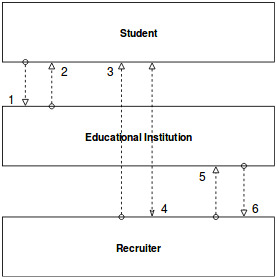
\includegraphics[width=0.8\textwidth]{Scenario1}
		\caption{Interactions in Scenario 1}
		\label{fig: Scenario1}
	\end{subfigure}
	%
	\begin{subfigure}[b]{0.3\textwidth}
		\centering
		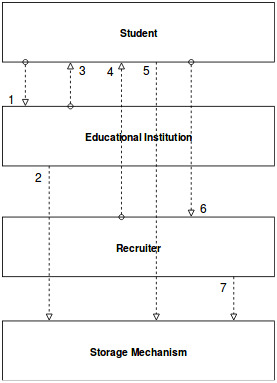
\includegraphics[width=0.8\textwidth]{Scenario2}
		\caption{Interactions in Scenario 2}
		\label{fig: Scenario2}
	\end{subfigure}
	%
	\begin{subfigure}[b]{0.3\textwidth}
		\centering
		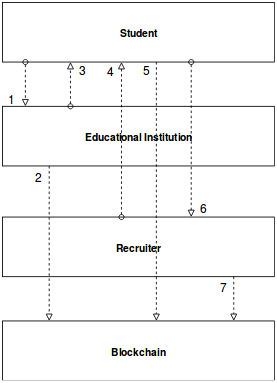
\includegraphics[width=0.8\textwidth]{Scenario3}
		\caption{Interactions in Scenario 3}
		\label{fig: Scenario3}
	\end{subfigure}

	\caption{Interactions presented to Respondents.}
\end{figure}

We used these actors as the basis to develop more complex scenarios and interactions, which we then used in our questionnaire. Respondents were presented with 3 interactions between these actors, as \gls{bpmn} \cite{BPMN} models, presented, respectively in Figure \ref{fig: Scenario1}, Figure \ref{fig: Scenario2} and Figure \ref{fig: Scenario3}. The context in which these interactions were presented is explained, in detail, in the forthcoming section. The three scenarios the respondents had to analyze described:
\emph{(i)} a typical scenario of issuing, sharing and validating an educational certificate, \emph{(ii)} a typical scenario, using an undisclosed storage mechanism, such as a database, with added access control functionality, and \emph{(iii)} a typical scenario, using a blockchain, with added access control functionality.



\subsection{Methodology}

This section discusses the methodology, used throughout the questionnaire, specifically the design of the questionnaire and its contents, and afterwards, the presentation and distribution methods are explained.

\subsubsection{Questionnaire Layout}

The questionnaire was designed to target professionals in multiple industries with different backgrounds and knowledge levels. It had 28 questions, of which 21 were mandatory questions and 7 were optional. There were 5 sections on the questionnaire: \textit{Introduction}, \textit{Background}, \textit{Exercise 1}, \textit{Exercise 2} and \textit{Final Survey}. There was no time limit nor were the respondents' participation offered any incentives. Participation was completely voluntary.

\subsubsection{Section Detail and Questions}

\textit{Introduction} explained the research objectives, the context in which it was inserted and it stated that all answers were anonymous and would only be used, and shared, for academic purposes.
%
\textit{Background} had four questions, with the aim of assessing respondents' professional and academic background, as well as their perceived knowledge of specific technologies and concepts. Those questions were:

\begin{enumerate}
	\item Do you have any academic or professional background related with Information Security?
	\item Which industry best fits with your professional experience?
	\item Which professional role best fits your experience?
	\item How do you classify your knowledge of the following concepts?
\end{enumerate}

In \textit{Exercise 1} and \textit{Exercise 2}, respondents were asked to answer specific questions. In \textit{Exercise 1} there were two separate scenarios to analyze. In \textit{Exercise 2} there was only one scenario to analyze. In each scenario, there was a simple \gls{bpmn} \cite{BPMN} model followed by a description of the interactions between the actors. All three scenarios had exactly the same 7 questions:

\begin{enumerate}
	\item Which level of security do you perceive in each interaction?
	\item Which level of security do you perceive in the entire process?
	\item What could make it more secure?
	\item Select any interactions you perceive as allowing unauthorized access to information being shared.
	\item If you were a Student, what would be your willingness to share information, in this context, with a Recruiter?
	\item  If you were a Student, what would be your confidence that the information you share is secure and no one, except the Recruiter, will access it?
	\item Which level of complexity do you perceive in each interaction?
\end{enumerate}

In the last section, \textit{Final Survey}, the respondents were asked two additional questions and a placeholder for some comments, if necessary:

\begin{enumerate}
	\item Do you think any of the previous 3 scenarios was more secure than the others?
	\item Do you believe knowledge of Information Security, its applications and concepts, is at an adequate level in your professional environment?
\end{enumerate}

Out of the 7 questions, in \textit{Exercise 1} and in \textit{Exercise 2}, 5 were based on Likert scales from 0 to 4, where 0 was the lowest possible value and 4 was the highest possible value. 1 question was an open-ended question - and 1 was a checkbox question. These questions, from each scenario - 21 questions in total - were the core of our study. The respondents were never asked to compare any scenario but only asked to answer the same questions for each scenario.

\subsubsection{Distribution Methods}

Two versions were made out of the same questionnaire. The first version had the following sequence: Typical scenario $\,\to\,$ Storage Mechanism scenario $\,\to\,$ Blockchain scenario. The second version had the following sequence: Storage Mechanism scenario $\,\to\,$ Typical scenario $\,\to\,$ Blockchain scenario. The questionnaire was made available online at a specific URL \footnote{https://hugomartins.io/human-perception-infosec/} and, upon clicking on it, respondents were redirected to one of the versions without knowing which version and without knowing that several versions existed. The aim of this separation was to try and mitigate the learning effect bias that might arise when analyzing the results of a questionnaire answered on a given sequence

The questionnaire was pretested with 1 respondent to validate there were no problems, before distribution and, after necessary corrections, was distributed. Distribution took place, initially, over email to a controlled group of 5 people to ensure the randomization system was working properly and that no errors occurred with submission, this was in order mitigate further problems before sending the questionnaire to more people. After that, it was sent, via email, to a group of 50 people, mainly professionals. That group grew to approximately 150 people. After that, the questionnaire was also posted on HackerNews \footnote{https://news.ycombinator.com/item?id=17064032}, as a LinkedIn post \footnote{https://www.linkedin.com/feed/update/urn:li:activity:6401809377023533056} and in Reddit: in /r/Assistance \footnote{https://www.reddit.com/r/Assistance/comments/8jk3hf/human\_perception\_of\_information\_security\_for} and /r/SampleSize  \footnote{https://www.reddit.com/r/SampleSize/comments/8jk5ej/academic\_human\_perception\_of\_information\_security}. The questionnaire was open for submission from May 9, 2018, until May 20, 2018. Overall, we were able to reach 82 views, of which 46 answered the questionnaire completely.

\section{Results}


This section presents the results of the questionnaire. We have analyzed both versions of the questionnaire separately, \textit{Version 1} and \textit{Version 2}, and performed a combined analysis, with both versions' data sets. This helps when discussing what it is possible to conclude from the results by taking into account possible learning effects' bias, as well as define the limitations that can be overcome in future work, discussed in Chapter \ref{chap:conclusion}.

This section is structured in direct relation to the design questions outlined, at the beginning of this chapter, by looking at the data that relates to each of them.

As described previously, 46 respondents answered the questionnaire, with 24 respondents answering \textit{Version 1} (52\%) and 22 respondents answering \textit{Version 2} (48\%). There was a balance between respondents with backgrounds related to Information Security - with 52\% of the respondents saying they do have a background related to Information Security. Nonetheless, in \textit{Version 1}, 62.5\% of the respondents said they did not have a background related to Information Security. Industries and Roles (see Table \ref{tab: industry} and Table \ref{tab: roles}) tended to be in the area of Software Development.

For simplicity of our analysis, we have corrected the switch made between \textit{Version 1} and \textit{Version 2}, when reporting the results, in order to allow a direct comparison between both data sets, instead of having to mentally compare them, using the sequence used in Version 1.

\begin{table}[htb]
	\centering
	\caption{Industry Frequency}
	\label{tab: industry}
	\begin{tabular}{l|c|c|c}
		\hline \bf Industry & \bf Version 1 & \bf Version 2 & \bf Both \\ \hline
		Consultancy         & 5             & 1             & 6        \\ \hline
		Telecom.            & 1             & 1             & 2        \\ \hline
		Software Dev.       & 9             & 15            & 24       \\ \hline
		R\&D                & 1             & 1             & 2        \\ \hline
		Academic            & 4             & 3             & 7        \\ \hline
		Other               & 2             & 1             & 3        \\ \hline
		N.A.                & 1             & 0             & 1        \\ \hline
		Health              & 1             & 0             & 1        \\ \hline
	\end{tabular}
\end{table}

\begin{table}[htb]
	\centering
	\caption{Role Frequency}
	\label{tab: roles}
	\begin{tabular}{l|c|c|c}
		\hline \bf Role  & \bf Version 1 & \bf Version 2 & \bf Both \\ \hline
		Software Dev.    & 13            & 12            & 25       \\ \hline
		Researcher       & 2             & 2             & 4        \\ \hline
		Professor        & 1             & 15            & 24       \\ \hline
		Business Manager & 5             & 1             & 6        \\ \hline
		Project Manager  & 1             & 4             & 5        \\ \hline
		Other            & 1             & 1             & 2        \\ \hline
		N.A.             & 1             & 0             & 1        \\ \hline
	\end{tabular}
\end{table}

Respondent's perceived knowledge of specific concepts, from 0 (lowest) to 4 (highest), slightly varied between versions, with \textit{Version 2} presenting a more knowledgeable set of respondents, in most concepts (see Table \ref{tab: knowledge}), with the concepts being: \emph{(i)} Access Control; \emph{(ii)} Encryption; \emph{(iiii)} blockchain; \emph{(iv)} Data Integrity; \emph{(v)} Malware; \emph{(vi)} Phishing; \emph{(vii)} Data Confidentiality; \emph{(viii)} \gls{bpmn}; \emph{(ix)} Data Storage; \emph{(x)} Unauthorized Access.

\begin{table}[htb]
	\centering
	\caption{Reported Knowledge Using the Scale 0 (Lowest) to 4 (Highest)}
	\label{tab: knowledge}
	\begin{tabular}{c|cc|cc|cc}
		\hline
		\bf Concept & \multicolumn{2}{c}{\bf Version 1} \vrule & \multicolumn{2}{c}{\bf Version 2} \vrule & \multicolumn{2}{c}{\bf Both}                                             \\
		\hline
		            & $\tilde{x}$                              & $\sigma_{x}$                             & $\tilde{x}$                  & $\sigma_{x}$ & $\tilde{x}$ & $\sigma_{x}$ \\
		\hline
		1           & 1.92                                     & 0.97                                     & 2.36                         & 1.18         & 2.13        & 1.09         \\
		\hline
		2           & 1.67                                     & 1.05                                     & 2.14                         & 1.13         & 1.89        & 1.10         \\
		\hline
		3           & 1.33                                     & 0.87                                     & 1.05                         & 0.84         & 1.20        & 0.86         \\
		\hline
		4           & 1.83                                     & 1.09                                     & 2.14                         & 1.21         & 1.98        & 1.15         \\
		\hline
		5           & 1.71                                     & 0.91                                     & 1.82                         & 0.96         & 1.76        & 0.92         \\
		\hline
		6           & 1.96                                     & 0.91                                     & 2.14                         & 0.94         & 2.04        & 0.92         \\
		\hline
		7           & 2.46                                     & 1.02                                     & 2.46                         & 1.01         & 2.46        & 1.01         \\
		\hline
		8           & 0.83                                     & 1.01                                     & 1.36                         & 1.36         & 1.09        & 1.21         \\
		\hline
		9           & 2.29                                     & 1.00                                     & 2.36                         & 1.33         & 2.32        & 1.16         \\
		\hline
		10          & 2.00                                     & 1.02                                     & 2.09                         & 1.27         & 2.04        & 1.13         \\
		\hline
	\end{tabular}
\end{table}

Regarding our background results, we can conclude that our sample tends towards Software Development, followed by professionals from Academia. This means that our sample is potentially more knowledgeable about common technology topics than a more mixed sample would. \textit{Version 1} respondents reported a below-average knowledge of the presented concepts, with a lower standard deviation, while \textit{Version 2} respondents reported a higher than average knowledge of the presented concepts, with a less concentrated set of answers. All coefficients of variation, in the compound analysis, are lower than 1 (between $C_v = 0.41$ and $C_v = 0.72$), except for \gls{bpmn} ($C_v = 1.11$). The same happens for each separate version, with different boundaries.

\subsection{Design Question 1}

\begin{quote}
	\textit{What is the perceived level of security in blockchain-based solutions, compared to other solutions?}
\end{quote}

To answer this question, we took special attention to questions 1, 2 and 4 of each of the scenarios. In questions 1 and 2, respondents were asked to evaluate the perceived security of a given scenario. The evaluations were for the process in its entirety and for each interaction in the scenario. Question 4 asked respondents to select the interactions they perceived as allowing unauthorized questions. We have also taken into consideration the answers given in the final question, in which respondents were forced to choose which scenario was the most secure.

Starting from the last question, an overwhelming majority of the respondents answered that they perceived the scenario using blockchain to be the most secure (see Table \ref{tab: mostSecure}) - when forced to choose.

\begin{table}[htb]
	\centering
	\caption{Most Secure Scenario (Total Amount of Responses)}
	\label{tab: mostSecure}
	\begin{tabular}{l|c|c|c}
		\hline \bf Answer & \bf Version 1 & \bf Version 2 & \bf Both \\ \hline
		None              & 1             & 1             & 2        \\ \hline
		Scenario 1        & 1             & 4             & 5        \\ \hline
		Scenario 2        & 3             & 3             & 6        \\ \hline
		Scenario 3        & 19            & 14            & 33       \\
		\hline
	\end{tabular}
\end{table}

This suggests that there's a tendency to believe that blockchain-based solutions are perceived as being more secure than other solutions. The fact that users were forced to choose one or none of the scenarios makes it more clear that, although we cannot claim any justification for it, respondents had a tendency to claim that blockchain-based solutions are more secure than other solutions. Even more interesting is that not only did respondents choose blockchain-based solutions against the typical scenario but the same occurred for the scenario that used a basic Storage Mechanism, instead of the blockchain-based one.

For the first question, which asked for the perceived level of security in each scenario (see Table \ref{tab: perceivedSecurity}), we witness similar results. We witness the same effect, in \textit{Version 2}, as we had previously, although the data is more spread (\textit{$\sigma_{x}$ = 1.23}).

\begin{table}[htb]
	\centering
	\caption{Perceived Security / Scenario Using the Scale 0 (Lowest) to 4 (Highest)}
	\label{tab: perceivedSecurity}
	\begin{tabular}{c|cc|cc|cc}
		\hline
		Scenario & \multicolumn{2}{c}{\bf Version 1} \vrule & \multicolumn{2}{c}{\bf Version 2} \vrule & \multicolumn{2}{c}{\bf Both}                                             \\
		\hline
		         & $\tilde{x}$                              & $\sigma_{x}$                             & $\tilde{x}$                  & $\sigma_{x}$ & $\tilde{x}$ & $\sigma_{x}$ \\
		\hline
		1        & 2.13                                     & 0.99                                     & 2.50                         & 1.23         & 2.30        & 1.11         \\
		\hline
		2        & 2.83                                     & 0.96                                     & 2.36                         & 0.95         & 2.61        & 0.98         \\
		\hline
		3        & 3.00                                     & 0.89                                     & 2.91                         & 0.87         & 2.96        & 0.87         \\
		\hline
	\end{tabular}
\end{table}

We can understand, by studying the coefficients of variation (Version 1: Scenario 1 ($C_v = 0.47$), Scenario 2 ($C_v = 0.34$), Scenario 3 ($C_v = 0.29$); Version 2: Scenario 1 ($C_v = 0.48$), Scenario 2 ($C_v = 0.40$), Scenario 3 ($C_v = 0.30$) that respondents' answers became more concentrated when it comes to blockchain-based solutions (Scenario 3), while being more dispersed in Storage Mechanism (Scenario 2) and even more in the typical process (Scenario 1). This further reinforces the appearing tendency.

By studying the results of the evaluation by interaction, in each scenario, and with the scenario as a whole, the data is less clear than previous answers. Results, seen in Table \ref{tab: perceivedInteractionSecurity}, have shown an increase in the dispersion of the data which impacts mean-based analysis. It is interesting that, contrary to what had happened when asked about the security of the entire process, in this case, in \textit{Version 1}, we cannot see a major difference between the results of Scenario 2 and Scenario 3. Nonetheless, we still see the same patterns as in the previous results, in \textit{Version 2} and when considering the data sets combined.

\begin{table}[htb]
	\centering
	\caption{Perceived Interaction Security / Scenario Using the Scale 0 (Lowest) to 4 (Highest)}
	\label{tab: perceivedInteractionSecurity}
	\begin{tabular}{c|cc|cc|cc}
		\hline
		Scenario & \multicolumn{2}{c}{\bf Version 1} \vrule & \multicolumn{2}{c}{\bf Version 2} \vrule & \multicolumn{2}{c}{\bf Both}                                             \\
		\hline
		         & $\tilde{x}$                              & $\sigma_{x}$                             & $\tilde{x}$                  & $\sigma_{x}$ & $\tilde{x}$ & $\sigma_{x}$ \\
		\hline
		1        & 2.26                                     & 1.30                                     & 2.58                         & 1.21         & 2.42        & 1.26         \\
		\hline
		2        & 2.71                                     & 1.13                                     & 2.27                         & 1.43         & 2.50        & 1.30         \\
		\hline
		3        & 2.68                                     & 1.12                                     & 2.72                         & 1.19         & 2.70        & 1.15         \\
		\hline
	\end{tabular}
\end{table}

In Figure \ref{fig: perceivedInteractionSecurityOne} we expose the data used to generate Table \ref{tab: perceivedInteractionSecurity}'s \textit{Version 1}, with line charts, in which the data sets for each scenario have been run through a probability density function. This allows us to see that the mean, for Scenario 2, is highly influenced by more skewed distributions and, at the same time, it confirms, visually, the data about the process as a whole. Scenario 3 is visually more secure and concentrated - the interactions perceived as more secure, individually.

\begin{figure}[htb]
	\centering
	\begin{subfigure}[b]{0.49\textwidth}
		\centering
		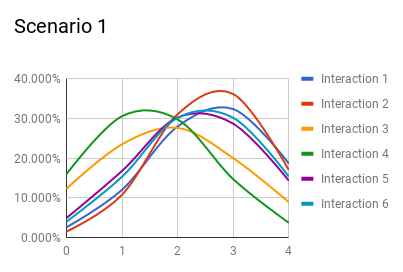
\includegraphics[width=\linewidth]{V1-S1-Security.png}
	\end{subfigure}
	%
	\begin{subfigure}[b]{0.49\textwidth}
		\centering
		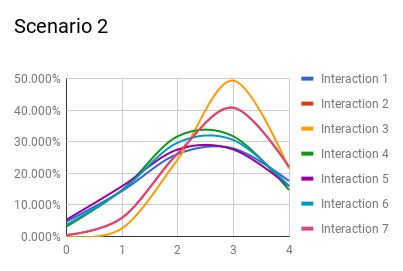
\includegraphics[width=\linewidth]{V1-S2-Security.png}
	\end{subfigure}
	%
	\hfill
	\begin{subfigure}[b]{0.49\textwidth}
		\centering
		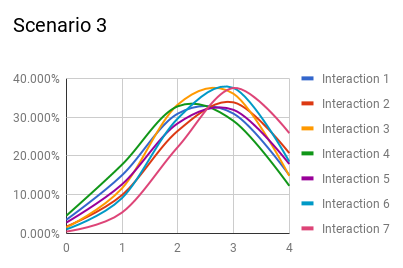
\includegraphics[width=\linewidth]{V1-S3-Security.png}
	\end{subfigure}

	\caption{Probability Density of Perceived Interaction Security (Version 1)}
	\label{fig: perceivedInteractionSecurityOne}
\end{figure}

At the same time, in Figure \ref{fig: perceivedInteractionSecurityTwo} we expose the data used to generate Table \ref{tab: perceivedInteractionSecurity}'s \textit{Version 2}. The visualizations closely resemble the one presented in Figure \ref{fig: perceivedInteractionSecurityOne}. This is relevant due to the fact that the aggregate numbers, shown in Table \ref{tab: perceivedInteractionSecurity}, only allow us to have a high-level understanding, of the respondents' perception. The visualizations help to understand that, even in more detail, the data is similarly distributed, although, somehow skewed to the left, in Scenario 1, and skewed to the right.

\begin{figure}[htb]
	\centering
	\begin{subfigure}[b]{0.49\textwidth}
		\centering
		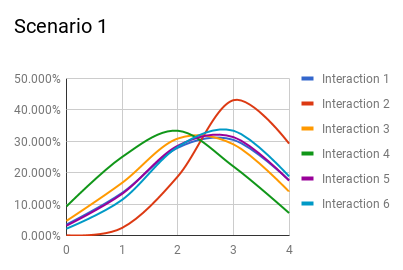
\includegraphics[width=\linewidth]{V2-S1-Security.png}
	\end{subfigure}
	%
	\begin{subfigure}[b]{0.49\textwidth}
		\centering
		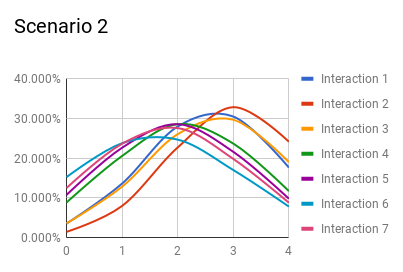
\includegraphics[width=\linewidth]{V2-S2-Security.png}
	\end{subfigure}
	%
	\hfill
	\begin{subfigure}[b]{0.49\textwidth}
		\centering
		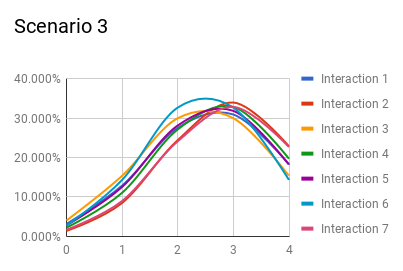
\includegraphics[width=\linewidth]{V2-S3-Security.png}
	\end{subfigure}

	\caption{Probability Density of Perceived Interaction Security (Version 2)}
	\label{fig: perceivedInteractionSecurityTwo}
\end{figure}

Finally, respondents also perceived that sharing the certificate, under a blockchain-based solution, had fewer interactions with the possibility of allowing unauthorized access to data, than with the typical purpose. The same is true for blockchain-based solutions over the Storage Mechanism.

\subsection{Design Question 2}

\begin{quote}
	\textit{What is the perceived complexity introduced by blockchain-based solutions?}
\end{quote}

\begin{table}[htb]
	\centering
	\caption{Perceived Complexity / Scenario Using the Scale 0 (Lowest) to 4 (Highest)}
	\label{tab: perceivedComplexity}
	\begin{tabular}{c|cc|cc|cc}
		\hline
		Scenario & \multicolumn{2}{c}{\bf Version 1} \vrule & \multicolumn{2}{c}{\bf Version 2} \vrule & \multicolumn{2}{c}{\bf Both}                                             \\
		\hline
		         & $\tilde{x}$                              & $\sigma_{x}$                             & $\tilde{x}$                  & $\sigma_{x}$ & $\tilde{x}$ & $\sigma_{x}$ \\
		\hline
		1        & 1.56                                     & 1.51                                     & 1.47                         & 1.13         & 1.51        & 1.14         \\
		\hline
		2        & 1.96                                     & 1.21                                     & 1.71                         & 1.25         & 1.82        & 1.23         \\
		\hline
		3        & 2.25                                     & 1.26                                     & 1.97                         & 2.00         & 2.12        & 1.24         \\
		\hline
	\end{tabular}
\end{table}

For this question, we have analyzed the answers to question 7 of each scenario, which asked respondents to grade each interaction they were shown, in terms of its complexity. We present the mean for all interactions' evaluation and also the standard deviation, per scenario (see Table \ref{tab: perceivedSecurity}). The results show that there's an increase in the perceived complexity of blockchain-based solutions. In this case, contrary to what happened with the previous design question, we do not see a pronounced learning bias as, regardless of the order of the questions, the tendency remained the same - and the compound analysis reflected that situation. It is also interesting to notice that, when asked about the concept of complexity, the dispersion of data increases, especially when compared to the concept of security.

\begin{figure}[htb]
	\centering
	\begin{subfigure}[b]{0.49\textwidth}
		\centering
		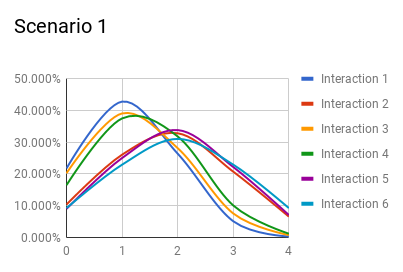
\includegraphics[width=\linewidth]{V1-S1-Complexity.png}
	\end{subfigure}
	%
	\begin{subfigure}[b]{0.49\textwidth}
		\centering
		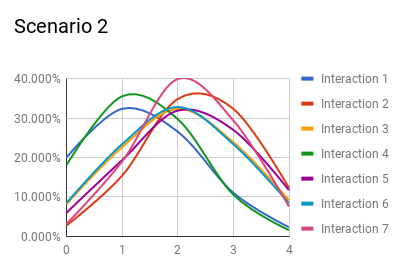
\includegraphics[width=\linewidth]{V1-S2-Complexity.png}
	\end{subfigure}
	%
	\hfill
	\begin{subfigure}[b]{0.49\textwidth}
		\centering
		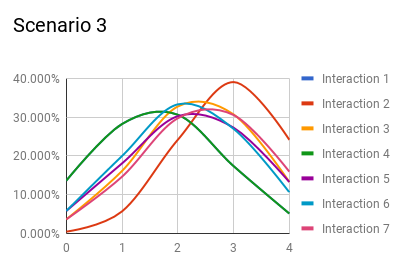
\includegraphics[width=\linewidth]{V1-S3-Complexity.png}
	\end{subfigure}

	\caption{Probability Density of Perceived Interaction Complexity (Version 1)}
	\label{fig: perceivedInteractionComplexityOne}
\end{figure}

\begin{figure}[htb]
	\centering
	\begin{subfigure}[b]{0.49\textwidth}
		\centering
		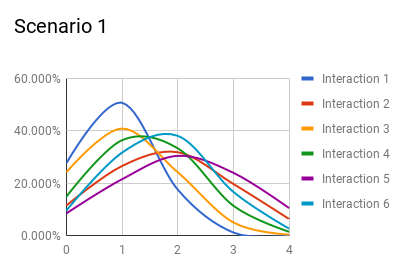
\includegraphics[width=\linewidth]{V2-S1-Complexity.png}
	\end{subfigure}
	%
	\begin{subfigure}[b]{0.49\textwidth}
		\centering
		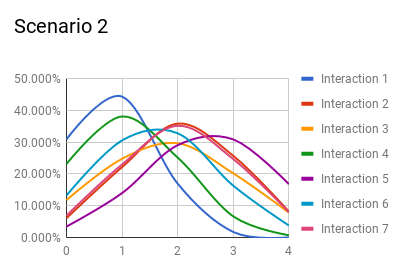
\includegraphics[width=\linewidth]{V2-S2-Complexity.png}
	\end{subfigure}
	%
	\hfill
	\begin{subfigure}[b]{0.49\textwidth}
		\centering
		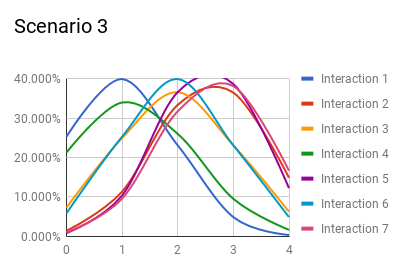
\includegraphics[width=\linewidth]{V2-S3-Complexity.png}
	\end{subfigure}

	\caption{Probability Density of Perceived Interaction Complexity (Version 2)}
	\label{fig: perceivedInteractionComplexityTwo}
\end{figure}

Figure \ref{fig: perceivedInteractionComplexityOne} and Figure \ref{fig: perceivedInteractionComplexityTwo} allow us to perform the same visual comparison, such as in the previous section. What we see indicates what has been shown in the high-level picture, both in terms of mean and standard deviation. For example, in the blockchain-based solutions (Scenario 3), in \textit{Version 2} , the data is very spread when compared inter-interaction but it seems to be much more concentrated for each interaction than in \textit{Version 1}.
\cleardoublepage

\chapter{Implementation}

\section{Framework for Access Control}

\section{Selected Technologies}


\section{Design and Architecture}

\section{\textit{blocked}}

\section{Summary}



\cleardoublepage

\chapter{Evaluation}

\section{Qualitative Evaluation}

\subsection{Guidelines for Access Control System Evaluation}

in this section, we evaluate our system through the metrics proposed in \cite{hu_guidelines_2012} which is a continuation from what has been presented in \cite{hu_assessment_2006}. Leveraging these metrics allows us to have an understading of what the access control systems is capable of executing.

\subsubsection{Administration Properties}

\begin{itemize}
	\item \textbf{Auditing}: \textit{blocked} audits the granting of access through the processing that happens inside the Transaction Processor. If the transactions submitted are approved, these are then stored in the blockchain. If, in turn, the transactions are rejected, the nodes will have a log that a given transaction has been rejected, along with the reason. At the same time, each client performs the needed validations for accessing a certificate, which means that denied read accesses won't be logged anywhere, except on the client node. The system does not provide additional log functions that can be customized and logging system failure can, also, only be done at the network level given the descentralized nature of the system. The auditing that gets stored is only per transaction, apart from all the information that can be stored in a transaction (such as allowing or revoking a given access), there are no more logs available.
	\item \textbf{Capabilities Discovery}: The system has lacking capabilities discovery functionality. It is not possible to discover capabilities of a given subject due to the fact that those capabilities are stored inside each certificate, spread throughout the blockchain. It is possible to discover which subjects have access to each cetificate, nonetheless. It is not possible to discovery any more information about each capability.
	\item \textbf{Ease of Privilege Assignments}: Assigning or removing a privilege is possible by executing the respective \textit{blocked} client. In both cases, it takes only one step to execute, apart from knowing the public identity of whoemever the privilege concerns. Updating a privilege is impossible. The system does not support the usage of group relations or inheritance.
	\item \textbf{Specifying AC Rules}: The system does not support the specification of AC rules nor can't it handle any rule specification logic.
	\item \textbf{Policy Management}: The system does not allow meta-policy information, expiration assignments, target event assignments, combinations for policies, policy distribution approval, management of policy authoritative sources or impact analysis. It does allow for target assignments, given that the default policy is directly assigned to a given target and it allows for runtime policy changes, in the sense that it allows a permission to be revoked during runtime.
	\item \textbf{Delegation of Administrative Capabilities}: No policy administration delegation is allowed. The system does not support it.
	\item \textbf{Flexibilities of Configuration into Existing Systems}: The access control is enforced via a combination of application logic, consensus protocols and cryptography. For viewing a certificate, a subject will need to possess the appropriate RSA private key, otherwise it won't be able to decrypt the data. For granting a permission, a subject also needs to have appropriate keys but, at the same time, needs to be either the issuer or recipient of a given certificate, otherwise the transaction will be rejected by the Transaction Processor running in the nodes.
	\item \textbf{Horizontal Scope of Control}: The system supports an array of hosts, each running its own Transaction Processor, that will connect via the network. Each node will have a copy of the entire blockchain.
	\item \textbf{Vertical Scope of Control}: The system covers application data that is store inside a blockchain. It does not cover any other scope of data.
\end{itemize}

\subsubsection{Enforcement Properties}

\begin{itemize}
	\item \textbf{Policy Combination, Composition, and Constraint}: The system allows only one policy and does not allow combination or composition of policies.
	\item \textbf{Bypass}: It is currently possible to bypass the system by changing the code of the Transaction Processor and running a changed version on the network. Nonetheless, it would still have to bypass the consensus of the network because it would be issuing invalid policies which would result in rejected transactions. On the viewer, it would be extremely had to bypass the system due to the fact that all the data is encrypted and secret keys, only known to the subjects, would be needed to bypass that data. Nonetheless, having those keys, one could bypass the system.
	\item \textbf{Least Privilege Principle}: Every subject is considered as having no access, unless it can decrypt one of the permissions, which means they have been granted access to that certificate. Granting access to a certificate grants access to only that certificate and no other on the system. At the same time, decrypting that certificate's symmetric key will prove useless when decrypting any other certificate because every certificate is encrypted with a different, randomly generated key.
	\item \textbf{Separation of Duty}: Since the system is based on a permissions-per-certificate model, it doesn't support separation of duties.
	\item \textbf{Safety}: There's a universal constraint on the system that states that only subjects that have the corresponding private keys, to the public keys that were granted access to. This prevents leakage of permissions. In case a permission is compromised, that permission should be revoked during runtime.
	\item \textbf{Conflict Resolution or Prevention}: The system does not support conflict resolution or prevention due to the fact that it doesn't allow policy definiton in such a way that it would generate conflicts.
	\item \textbf{Operational/Situational Awareness}: The system does not support this. At the same time, this functionality doesn't fit the model that has been defined.
	\item \textbf{Granularity of Control}: The system only supports defining the granularity to the certificate object, it doesn't support any other finer-grained controls.
	\item \textbf{Expression Properties}: The system does not support expressing policy, rule specification languages, rule composing using standards or rule combinations.
	\item \textbf{Adaptable to Evolution of AC Policies}: The system does not support adapting to evolution because it only supports a single policy.
\end{itemize}

\subsubsection{Performance Properties}

\begin{itemize}
	\item \textbf{Response Time}: \textcolor{red}{EXPERIMENTAL EVALUATION}
	\item \textbf{Policy Repository and Retrieval} - \textcolor{red}{EXPERIMENTAL EVALUATION}
	\item \textbf{Policy Distribution}: Policy is distributed through a consensus protocol to all the nodes in the network, after each has validated the transaction, the data is updated accordingly in their blockchain.
	\item \textbf{Authentication}: Authentication is performed on the basis of public key criptography, through the usage of public keys as identities.
\end{itemize}

\subsubsection{Support Properties}

\begin{itemize}
    \item \textbf{Policy Import and Export}: The system does not support import, export or convertion of access control policies.
    \item \textbf{OS Compatibility}: The system supports only Ubuntu 18.04 LTS.
    \item \textbf{Policy Source Management}: The system does not use authorative sources, given that one of the goals is descentralizing the system thus having no single authority, and, for that, does not support source management.
    \item \textbf{User interfaces and API}: The system provides only command line user interfaces for interaction with the system.
    \item \textbf{Verification and Compliance Function}: The system does not provide verification and compliance functionalities.
\end{itemize}

\section{Quantitative Evaluation}




\cleardoublepage

\chapter{Conclusion}
\label{chap:conclusion}

We explored whether usage of permissioned blockchain would provide a solution for decentralization of access control, in the context of issuing, sharing and managing digital Educational Certificates. This problem emerges from the intersection of an increasingly distributed technological landscape, an increase in the amount in generation of digital information, the increase in the adoption of MOOC-based learning and the lack of tools for practical issuance and verification of those learning certificates. Previous research had provided options that are either not entirely decentralized, required complex \gls{pki} to use, lack integration with permissioned blockchains or are missing access control functionality, that allows users to control who accesses what information. We have sought, with this research, to explore whether building a system on top of a permissioned blockchain would allow us to provide those guarantees of decentralization.

We have started by performing a statistical study in order to assess how users perceive blockchain-based technologies, in terms of security and complexity, and applications built on top of those, in order to assess the adoption that our proposed approach could potentially have. At the same time, we used that questionnaire to try and guide the design and architecture of the system that has been proposed. This initial step, guided by our choice of using \gls{dsrm}, as our research methodology, allowed us to cautiously conclude that our proposed solutions has potential in terms of user's adoption and is a small step towards resolving the presented issues.

With that in mind, we designed a system \texttt{Blocked}, based on the concept of permissioned blockchains, to issue, share and manage Educational Certificates. This system relies on a permissioned blockchain platform, specifically Hyperledger Sawtooth, and cryptography-based permissions to allow decentralization of policy distribution, maintaining integrity and privacy of information stored inside the blockchain. \texttt{Blocked} has been developed to be used on a peer-to-peer network, where each node might be responsible for validating the current state of the blockchain. Apart from cryptography-based permissions, \texttt{Blocked} also allows for configuration of permissions at the network level, based on the identities of the nodes participating in the network, which is specially suitable from an organizational perspective.

Finally, we have proved our concept through implementing the proposed design and running a simulation. We have also described how the implemented system fits in with the responsibilities of an access control system. This system is not meant to be a replacement for existing solutions (such as \emph{BlockCerts}) but rather it is meant to show an alternative way of solving the decentralization system, that is more suitable for specific use cases. We have also evaluated how the results of our exploratory statistical study describe potential impacts on the future study of blockchain-based research.

\section{Contributions}

According to what has been described previously, our stated goal of exploring decentralization of access control through the usage of permissioned blockchains, this thesis produced an artifact in order to resolve that issue.

Our main contribution is the \texttt{Blocked} system design, architecture and implementation, along with a proof-of-concept. This contribution, along with its evaluation, demonstrates that there's a real potential in using permissioned blockchains for decentralizing access control, in the context o issuing, sharing and managing Educational Certificates.

A minor contribution, that was intrinsically connected with our major contribution, was the statistical study performed, in order to assess users' perceptions of blockchain-based technologies, in terms of security and complexity. The results have indicated a tendency for users to perceive blockchain technology as more secure but, alas, more complex too. We have evaluated the potential of these findings, in developing future applications relying on blockchains, during these thesis.

\section{Future Research}

The contributions described in this thesis can be extended, or adapted, in different directions through future research. We have explored some of the limitations of this thesis, in a previous chapter, and those limitations are a guide to some of the directions in which this research could be extended. All of these extensions should, nonetheless, be focused on improving the applicability of these contributions to real-world scenarios and applications, rather than simulations.

It would be interesting to expand on the results of the statistical study described in this thesis. This extensions should have 3 major focuses: increasing the number and diversity of participants; experimenting with different versions of questionnaires, to rule out a learning bias in the results; and use different platforms and methodologies (such as interviews instead of questionnaires) to \emph{(i)} reproduce the results and \emph{(ii)} gain a deeper understanding of user's perceptions on these topics. This would allow us to improve on the development workflows used to build blockchain-based applications.

Another interesting extension would be to refine the design and architecture of \texttt{Blocked}. This should be done in different ways, overcoming the limitations described previously, by: further evaluating the \gls{poet} consensus algorithm; developing a more generalized system that would be decoupled from Hyperledger Sawtooth, being able to support other permisisoned blockchain platforms; and improving on some of the aspects of privacy mentioned in the limitations.

Finally, improving the overall implementation provided in this thesis. This can be done by providing packaged solutions for ease of use, providing a \gls{gui} and improving usability of the artifact. At the same time, more experiments need to be done with different network configuration, different testbeds and real-world simulations, in order to continously assess the performance of the system.

These suggestions of extensions are meant to focus future research on improving the existing prototype proof-of-concept implementation and design into a real-world production application that can have a practical impact on the problem we set out to explore.





\cleardoublepage

% -------------------------------------------------------
% References
% -------------------------------------------------------

\phantomsection
\addcontentsline{toc}{chapter}{References}
\printbibliography[title=References]

\end{document}
